\RequirePackage[l2tabu,orthodox]{nag}

% TODO: decide if one-sided/two-sided
%\documentclass[headsepline,footsepline,footinclude=false,fontsize=11pt,paper=a4,listof=totoc,bibliography=totoc,BCOR=12mm,DIV=12]{scrbook} % two-sided
\documentclass[headsepline,footsepline,footinclude=false,oneside,fontsize=11pt,paper=a4,listof=totoc,bibliography=totoc]{scrbook} % one-sided

% !TeX root = main.tex

\usepackage{graphicx}
\usepackage{amsmath}
\usepackage{tikz}
\usepackage[%
	backend=biber,
	url=false,
	style=numeric,
	maxnames=4,
	minnames=3,
	maxbibnames=99,
	giveninits,
	uniquename=init]{biblatex}
\usepackage{pgfpages}
\usepackage{multicol}
\usepackage{multirow}
\usepackage{appendixnumberbeamer}

\bibliography{bibliography}

\newcommand{\labelname}[1]{
	\def\insertenumlabel{#1}%
	\usebeamertemplate{enumerate item}%
}

\usefonttheme[onlymath]{serif} % use classic math font

\setcounter{secnumdepth}{1} % only sections for table of contents
\setcounter{tocdepth}{1}

\beamertemplatetransparentcoveredmedium
\beamertemplateballitem
\beamertemplatebookbibitems
\usenavigationsymbolstemplate{} % hide controls
\setbeamertemplate{footline}[frame number]
\usetheme{default} % plain white with blue headings

\setbeamertemplate{footline}
{
	\leavevmode%
	\hbox{%
		\begin{beamercolorbox}[wd=.333333\paperwidth,ht=2.25ex,dp=1ex,center]{author in head/foot}%
			\usebeamerfont{author in head/foot}\insertsection
		\end{beamercolorbox}%
		\begin{beamercolorbox}[wd=.333333\paperwidth,ht=2.25ex,dp=1ex,center]{title in head/foot}%
			\usebeamerfont{title in head/foot}\insertsubsection
		\end{beamercolorbox}%
		\begin{beamercolorbox}[wd=.333333\paperwidth,ht=2.25ex,dp=1ex,right]{date in head/foot}%
			\usebeamerfont{date in head/foot}\insertshortdate{}\hspace*{2em}
			\insertframenumber{} / \inserttotalframenumber\hspace*{2ex}
	\end{beamercolorbox}}%
	\vskip0pt%
}

\usefonttheme{structurebold}

\usecolortheme{rose} % orchid for a more dark version
\definecolor{orange}{rgb}{1,.549,0}
\definecolor{pink}{rgb}{1,0.5,0.5}
\definecolor{green}{rgb}{0,0.5,0}

% hide steps
\setbeamercovered{invisible}

% Tiny bib and add labels
\renewcommand*{\bibfont}{\scriptsize}
\setbeamertemplate{bibliography item}{\insertbiblabel}

\newcommand*{\getUniversity}{Technische Universität München}
\newcommand*{\getFaculty}{Department of Informatics}
\newcommand*{\getTitle}{A Tool Architecture for the Continuous\\\vspace{2mm} Detection of Open-Source License Infringements using Clone Detection} 
\newcommand*{\getTitleGer}{Werkzeugarchitektur zur kontinuierlichen Erkennung von Verstößen gegen Open-Source-Lizenzen durch Clone Detection}
\newcommand*{\getAuthor}{Benedikt Schlagberger}
\newcommand*{\getDoctype}{Master's Thesis in Informatics}
\newcommand*{\getSupervisor}{Prof. Dr. Dr. h.c. Manfred Broy}
\newcommand*{\getAdvisor}{Dr. Martin Feilkas}
\newcommand*{\getSubmissionDate}{15. January 2018}
\newcommand*{\getSubmissionLocation}{Munich}

\begin{document}

% Set page numbering to avoid "destination with the same identifier has been already used" warning for cover page.
% (see https://en.wikibooks.org/wiki/LaTeX/Hyperlinks#Problems_with_Links_and_Pages).
\pagenumbering{alph}
\begin{titlepage}
  % HACK for two-sided documents: ignore binding correction for cover page.
  % Adapted from Markus Kohm's KOMA-Script titlepage=firstiscover handling.
  % See http://mirrors.ctan.org/macros/latex/contrib/koma-script/scrkernel-title.dtx,
  % \maketitle macro.
  \oddsidemargin=\evensidemargin\relax
  \textwidth=\dimexpr\paperwidth-2\evensidemargin-2in\relax
  \hsize=\textwidth\relax

  \centering

  \IfFileExists{logos/tum.pdf}{%
    
\includegraphics[height=20mm]{logos/tum.pdf}
  }{%
    \vspace*{20mm}
  }

  \vspace{5mm}
  {\huge\MakeUppercase{\getFaculty{}}}\\

  \vspace{5mm}
  {\large\MakeUppercase{\getUniversity{}}}\\

  \vspace{20mm}
  {\Large \getDoctype{}}

  \vspace{15mm}
  {\huge\bfseries \getTitle{}}

  \vspace{15mm}
  {\LARGE \getAuthor{}}

  \IfFileExists{logos/faculty.pdf}{%
%    \vfill{}
    
\includegraphics[height=20mm]{logos/faculty.pdf}
  }{}
\end{titlepage}


\frontmatter{}

\begin{titlepage}
  \centering

  \IfFileExists{logos/tum.pdf}{%
    
\includegraphics[height=20mm]{logos/tum.pdf}
  }{%
    \vspace*{20mm}
  }

  \vspace{5mm}
  {\huge\MakeUppercase{\getFaculty{}}}\\

  \vspace{5mm}
  {\large\MakeUppercase{\getUniversity{}}}\\

  \vspace{20mm}
  {\Large \getDoctype{}}

  \vspace{15mm}
  {\huge\bfseries \getTitle{}}

  \vspace{10mm}
  {\huge\bfseries \foreignlanguage{ngerman}{\getTitleGer{}}}

  \vspace{15mm}
  \begin{tabular}{l l}
    Author:          & \getAuthor{} \\
    Supervisor:      & \getSupervisor{} \\
    Advisor:         & \getAdvisor{} \\
    Submission Date: & \getSubmissionDate{} \\
  \end{tabular}

  \IfFileExists{logos/faculty.pdf}{%
    \vfill{}
    
\includegraphics[height=20mm]{logos/faculty.pdf}
  }{}
\end{titlepage}

\thispagestyle{empty}
\vspace*{0.8\textheight}
\noindent
I confirm that this \MakeLowercase{\getDoctype{}} is my own work and I have documented all sources and material used.

\vspace{15mm}
\noindent
\getSubmissionLocation{}, \getSubmissionDate{} \hspace{50mm} \getAuthor{}

\cleardoublepage{}

\addcontentsline{toc}{chapter}{Acknowledgments}
\thispagestyle{empty}

\vspace*{20mm}

\begin{center}
{\usekomafont{section} Acknowledgments}
\end{center}

\vspace{10mm}
First, I would like to thank my thesis advisors Dr. Martin Feilkas for inspiring me and Dr. Benjamin Hummel for his perseverance, time and support during the whole time I wrote this thesis.
Also, I want to thank Prof. Manfred Broy for agreeing to supervise me.

I would also like to acknowledge my fellow students and friends Nils Kunze, Thomas Pettinger and Fabian Denbsky for proofreading this thesis, and I am gratefully indebted to their very valuable comments.
A special thanks goes out to my friends and roommates Albert Steckermeier and Viktoriia Rakytianska for proofreading, giving me useful advices and helping me out, whenever I had questions.

Furthermore, I would like to thank my colleagues at CQSE GmbH for supporting me when I had questions and giving me the opportunity to write and work in a gracious and welcoming working environment.

Finally, I must express my gratitude to my parents and to my girlfriend Isabella Fageth for providing me with unfailing support and continuous encouragement throughout my years of study and through the process of researching and writing this thesis.
This accomplishment would not have been possible without them.

\cleardoublepage{}

\chapter{\abstractname}
Open source code shared on platforms like GitHub or BitBucket is often licensed for modification and reuse even in commercial systems.
Permissive licenses usually demand to inform about the origin of the code, whereas more strict ones like the GNU Public License (GPL) or other copy-left licenses require developers to distribute software which relies on the code as open source under the same license or terms.
When copy-left code is copied into a close-sourced code base, the license scheme is violated and the company owning the codebase may face huge fines, when the violation is revealed.

In this thesis, a tool for the continuous detection of open source code in a codebase is developed.
The client-server architecture proposed uses techniques known from clone-detection to create an index, which holds cloning information on huge amounts of freely available open source code on the server-side.
Besides offering a service for querying similar code, the server also generates a bloom filter, which can be downloaded by clients and is used to increase the speed of the search process and reduce the load on the server.
To increase the accuracy of the detection, the history of the indexed projects is also taken into account.

The approach is prototypically implemented and evaluated by indexing 2.000 open source projects of different languages and analyzing 20 projects for copied code, resulting in a total database size of 37 GB and filters of less than 200 MB.
In 25\% of the analyzed projects, licensing issues could be found by manual inspection.
However, automation of the process is hard, because determining the origin and license of files in open source projects is very difficult.
\chapter{Zusammenfassung}
Open-Source-Software, welche auf Plattformen wie GitHub oder BitBucket veröffentlicht wird, ist oft so lizenziert, dass sie sogar in kommerziellen Systemen wiederverwendet werden kann.
Freizügige Lizenzen fordern im Fall einer Wiederverwendung nur eine Quellenangabe, wohingegen strengere Lizenzen wie die GNU General Public License (GPL) oder andere Copyleft Lizenzen verlangen, dass darauf aufbauender Code unter derselben Lizenz veröffentlicht werden muss.
Wird dennoch lizenzierter Quellcode ohne Quellenangabe verwendet oder in inkompatibel lizenzierte Softwaresysteme übernommen, wird entsprechend die Lizenz des Originalcodes verletzt.
Die Autoren müssen dann ihre Software entsprechend kennzeichnen oder gegebenenfalls sogar als Open Source veröffentlichen.

In dieser Arbeit wird ein Werkzeug entwickelt, welches aus Open-Source-Systemen kopierten Quellcode in einer Codebasis erkennen kann.
Dabei indexiert der Server eine sehr große Anzahl an Open-Source-Systemen und deren Historie.
Er stellt eine Schnittstelle zur Verfügung, welche es ermöglicht, nach Quelltextpassagen mit sehr hoher Ähnlichkeit zu suchen.
Der Server berechnet außerdem eine Filterstruktur, welche von Clients heruntergeladen und benutzt werden kann, um den Suchvorgang enorm zu beschleunigen.
Dies vermindert zudem die Auslastung des Servers.

Der Ansatz wurde prototypisch umgesetzt und bezüglich seiner Performanz untersucht.
Dafür wurden 2.000 Open-Source-Projekte in zwei verschiedenen Sprachen indexiert und anschließend mithilfe des Index 10 weitere Projekte jeder Sprache auf kopierten Quellcode untersucht.
Die erzeugte Datenbank ist ca. 37 GB groß, die Größe des Filters beträgt etwa 200 MB.
Durch manuelle Inspektion wurden in 25\% der analysierten Projekte Lizenzprobleme entdeckt.
Eine Automatisierung des Prozesses ist jedoch sehr kompliziert, da es sehr schwierig ist, die Lizenz einer Datei richtig zu ermitteln.
\microtypesetup{protrusion=false}
%TODO \setcounter{tocdepth}{1} 
\tableofcontents{}
\microtypesetup{protrusion=true}

\mainmatter{}

% !TeX root = ../main.tex

\chapter{Introduction}\label{chapter:introduction}
blabla motivation

To fight these problems, in this work a architecture for tool should be developed, which allows to search a codebase for copied code from open source software available on the Internet.
The approach of this work is a server system which holds a search engine for code.

Client server, because of updates and huge database. Index can not be downloaded for every update

%TODO See Title of work!!!

\section{Use cases}\label{section:introduction/use_cases}
As mentioned above, detection of license infringement is one use case for the tool.
Beside that, the tool can also be used to...
\begin{itemize}
	\item Prevent license infringement
	\item Link lib instead of copy is the better approach. This also ensures that the library can be exchanged and updated if vulnerabilities are discovered in its code.
	\item This brings the next point: Vulerabilities in the copied code
\end{itemize}

\section{Research Questions}\label{section:introduction/research_questions}
This work should answer the following research questions:
Is it possible to index huge amounts of sourcecode equivalent ot the size of all open source systems available on the Internet?
How big would such an index be relative to the amount of scanned code?
When, scanning a codebase, in which detail does the history has to be scanned as well? %Commit-based? Tag based?
Is it possible to 
%TODO ref Ausschreibung

% digital content -> easily copied

% TODO content of thesis:
First, the current state of research is reflected.
% !TeX root = ../main.tex

\chapter{Preliminaries}\label{chapter:preliminaries}
This chapter presents preliminaries for this work and term definitions which are used in the following chapters.
First, terms used throughout this work are listed and explained.
Second, the term \enquote{license infringement} in the context of the developed detection tool is defined and the impact on decisions during the development process are presented.
Lastly, the term code cloning and its relation to this work are explained.

\section{General Terms}\label{section:preliminaries/terms}
The following list contains terms which are used throughout this work.

\begin{description}
	\item[Reference System/Project]
		A codebase which can be detected by the tool. 
		Files of the reference system have to be analyzed by the tool and information about the code has to be extracted and stored.
	\item[Target System/Project]
		A codebase which is analyzed for license infringements by the tool.
		Code which is copied from a reference system to the target system should be found and its similarity assessed.
	\item[Clone Index] 
		A database which allows quick querying for similar code.
		In this work, a key-value store is used, which stores a value under some key, usually a hash of the value.
		The process of analyzing a source code files and storing cloning information into the index is called indexing.
	\item [Bloomfilter]
		A space efficient data structure which can tell whether an element is part of a set with a high probability. 
		False positives are possible, false negatives are not.
		The probability for a false positive can be calculated. 
		See \autoref{section:approach/creating_index/hash_filter} for more details.
	\item [Chunk]
		A sequence of statements with specific length extracted from a source code file.
		This segmentation is used to find matches between files of a target and a reference system.
	\item [Match]
		A linking between a chunk in a target system whose hash matches the hash of one or more chunks in a reference system.
\end{description}

\section{License Infringements}\label{section:preliminaries/infringement}
The first and primary use case of the tool developed in this work is to detect copy-pasted open source code and uncover licensing issues.
Here, several question arise:

\subsection*{How much copied code can cause a license infringement?}\label{section:preliminaries/infringement/how_much_code}
Gabel and Su did some analysis regarding the uniqueness of code.
Their study \enquote{revealed a general lack of uniqueness in software at levels of granularity equivalent to approximately one to seven lines of source code'} \cite{2010-gabel-su-source-code-uniqueness}.
Thus, the smallest size of a clone which can be argued as a license infringement should be set at 8 lines of code.

In a lawsuit case explained by Mertzel \cite{mertzel2008copying}, 54 lines of code (0,03\% of the codebase) where found and judged as copied code.
Consequentially, a detected clone should be seen as a serious violation when it reaches a length of 54 lines of code or more.

\subsection*{Which licenses are relevant for detection?}\label{section:preliminaries/infringement/relevant_licenses}
The answer for this question decides whether specifically licensed open source code should be detected by the tool.
There are many different open source licenses which all try to cover a different purpose.
A list of many common open source licenses and their properties can be found in \cite{licenses}.
In the context of this work, licenses are separated into three different categories:

\begin{description}
	\item[Restrictive Licenses] Licenses which do not permit use without permission by the author or in the given environment.
		This can be a copyright, which is default when no license is declared.
		Another example are copy-left licenses, like the GNU Public License (GPL), which forces software authors to license derivative work under the same license and can therefore cause licensing issues, when reused in closed-source codebases.
	\item[Permissive Licenses]
		Licenses which allow modification and use with conditions.
		Conditions may be that the derivative work has to attribute the used code or patent right regulations.
		Examples are the Apache, MIT or some forms of the BSD License.
	\item[Public Domain] 
		Code under public domain or under licenses like Unlicense, which allows use without any conditions, except that the creator does not provide any warranties and can not be held responsible for any damages or other liabilities.
\end{description}

Regarding the purpose of the tool developed in this work, all licenses except the last category may be of interest since not listing the use of a source under a permissive license can already be an infringement.
It can also be argued that code under public domain should be detected as well, since linking external code is enhancing maintainability compared to copy-pasting \cite{heinemann2012effective}.
\\ \\
\noindent
One problem in the context of this work are codebases with files which have a different license, than the codebase itself.
This is for example relevant, if code of a permissive license is copied into a codebase under a restrictive license.
For the development of the tool, the difficulty is to classify the file correctly into the right license category defined above.
Developing an automated approach for detecting the exact origin and consequentially the license is beyond the scope of this work.
Therefore, manual inspection of matches between a target's and reference system's file is mandatory for decision making.

\section{Code Cloning}\label{section:preliminaries/code_cloning}
For this work, code has to be compared and its similarity assessed.
A lot of work has been done in this area, starting more than 30 years ago \cite{lancaster2004comparison}.
During that time, terms specifying the similarity of code have been established.

In general, sections of similar code which may have been caused by copying the code are called \textit{clones}.
In this context ``similar'' can be anything between a 1:1 copy over small differences like variable renaming up to clones which only have a somewhat similar structure or produce the same output for a given input.
The similarity of clones can be categorized into different types, according to \cite{roy2007survey}:

\begin{description}
	\item[type-1] Identical code fragments except for variations in whitespace (may be also variations in layout) and comments.
	\item[type-2] type-1 clones and structurally/syntactically identical fragments except for variations in identifiers, literals, types, layout and comments.
	\item[type-3] type-2 clones and copied fragments with further modifications. Statements can be changed, added or removed in addition to variations in identifiers, literals, types, layout and comments.
	\item[type-4] type-3 clones and two or more code fragments that perform the same computation but are implemented through different syntactic variants.
\end{description}

However, those clone types are just a reference.
For clone detection tools it makes sense not to concentrate on one specific clone type, but rather on the purpose of the tool and the similarity of clones has to be defined in more detail.
This also is true for this work.
 
\subsection*{Which clones are relevant for license infringements?}
The goal of this work is to find code which has been copied from source code available on the Internet and my cause licensing issues.
Code is copied for many reasons, e.g. to save time and effort, because of a lack of knowledge, difficulty of understanding etc. \cite{roy2007survey}.
Instead of implementing the functionality from scratch, code which is already available to the developer is used, which may include code available as open source software on the Internet.
Because the code may also be difficult to understand or time might be tight, it is copied rather untouched.
This would result in a similarity comparable to a type-1 clone.

In copies which should be detected by the tool developed in this work, small modifications may have been done e.g. added lines for logging purposes.
This would result in a gapped clone, where a single type-1 clone is split up into multiple type-1 clones due to changed, added or removed lines, which is the clone type targeted in this work.
% !TeX root = ../main.tex

\chapter{Related Work}\label{chapter:related_work}
Lots of research has been done in the area of detecting copy-pasted code.
This mainly results from the huge field of application, where such techniques can be used.
Most of the research can be differentiated in the types of copied code which they detect.
In the case of this work, code which differs in formatting and small added/removed or rearranged statements are of advantage since developers may change the copied code slightly or add print statements.

\section{Detecting Similarities in Source Code}\label{section:related_work/detecting_similarities}
On of the earlies areas is detection of copy-pasted code in student submissions of programming lessons, which is researched since more than 30 years\cite{lancaster2004comparison}.
String and token based approaches like YAP3\cite{wise1996yap3}, JPLAG\cite{prechelt2002finding} or MOSS\cite{schleimer2003winnowing} use greedy-string-tiling, sometimes in combination with anagrams, to find similarities in files.
Other approaches like dup\cite{baker1995finding}, SID\cite{chen2004shared} or GPLAG\cite{liu2006gplag} build a data structures which represents the structure of the programs.
Those structures are then used to compare the programs.

Student submissions are usually aiming for a solution to a common given problem.
When students copy code for such submissions, they often try to trick the plagiarism detection tools by modifying the copied code.
Because of that, those tools are developed for finding copied code in programs where similarities are expected and therefore concentrate on detecting the potential amount of copy-pasting.
They try to detect clones with heavy modifications like rearranged, added, removed or changed statements.
The purpose of this thesis however, is a little different.
This work concentrates on finding copied code which is easily recognized as such, when seen side-by-side.

\section{Clone Detection}\label{section:related_work/clone_detection}
Another area is the detection of clones in the context of code quality.
Clones are two or more similar sections in code mainly originating from copy-pasting.
% Difference compared to \ref{section:related_work/detecting_similar_code}

One of the tools widely known and used is the one from Kamiya et al. called CCFinder\cite{kamiya2002ccfinder} which features a suffix-tree based approach.
They first transform the code by modifying language dependent syntax (e.g. remove accessibility keywords in Java).
After that, they divide the code into token sequences.
Those tokens are further transformed by replacing variable names and literals.
Now the suffix-tree is built over the token sequences. 
With that it is possible to easily find similar token sequences by traversing the tree down to a leave, which points to a location in a file.

Hummel et al.\cite{hummel2010index} developed an approach, where chunks of code are hashed.
They first tokenize the code and normalize it by removing e.g. comments and unifying variable names.
Now the tokens are split into statements, several of them are grouped into chunks and hashed.
When the hash value is calculated the same way for another section of code, it can be used to look up similar code sequences.

Koschke et al. \cite{koschke2014large,koschke2012large} tried to find license infringements in code.
Using a suffix-tree, they showed that this approach is faster than an index based one.
However, \glqq evaluation shows that [their] approach is faster than index-based techniques when the analysis is run only once. If the analysis is to be conducted multiple times, creating an index pays off\grqq \cite{koschke2014large}.

Sajnanj et al. \cite{sajnani2016sourcerercc} and Svajlenko and Roy \cite{svajlenko2017fast} developed a workbench for large scale clone detection.
In their work, they split blocks of code into tokens and sort them by frequency of use.
Caclulating the overlap coefficient for blocks is used to assess their similarity.
They could find clones in 250 million lines of code within 4 days, which is significantly faster than other clone detection tools at the time.

Both, using a suffix-tree or a index for finding copied code, may be suiting the requirements of the tool developed in this thesis.
However, a suffix-tree is quite difficult to persist and share between machines.
The advantage of a index in the context of this work is the possibility to extract certain information which can be used to decide whether an element is part of the index.
%TODO is scheiße, überarbeiten!

\section{Code Search}\label{section:related_work/code_search}
With the growth of the Internet, recent research areas start to aim for search engines for code.
Search engines like Google are good for string based searches, but bad for searching program structure.

Bajracharya et al. tried to fill the gap and developed a search engine for open source code.
They extract additional information from the code such as entities (package, interface, class, declarations, ...), relations (dependencies between classes, files, ...), keywords and fingerprints (structures, types, patterns, ...).
This information is then used to query the database and find code which matches the specified properties.

Keivanloo et al. tried to develop a linked-data repository called SeCold \cite{keivanloo2012leveraging,keivanloo2011internet,keivanloo2011seclone,keivanloo2010semantic}.
The system has different parts which enable a user to search for code clones, similar bytecode or program structure.
The most interesting part of the system in the context of this thesis is the clone search called SeClone, which is described in \cite{keivanloo2011internet,keivanloo2011seclone}.
For preprocessing, they first tokenize the code using ASTs (Abstract Syntax Tree) and a normalization approach similar to CCFinder as described in \cite{kamiya2002ccfinder}.
For indexing, the tokens are feed into two different databases, one for code patterns and one to store type usage which is for reducing the amount of false positives.
To enable detecting clones with added, changed or removed statements, they use a multilevel indexing approach, where lines of code are hashed, the emerging hashes sorted and after that, hashes for multiple lines are hashed again.
This multilevel approach allows rearranging of statements still resulting in the same hash for the code section and can detect type 3 clones.
Also, it improves the speed when searching for clones to the microseconds range.

Although those approaches fit the requirement of collecting huge amounts of code in a database and making it searchable, they aim for finding all code by its structure.
In this work, the goal is to find code which is copy-pasted and only modified slightly, if at all.

\section{Commercially Available Tools}
There are several commercially available tools, namely Blackduck and Flexnet Code Insight.
Both are advertised as able to detect code of freely available open source software (FOSS) in a given codebase.
This enables the user to be notified of possible vulnerabilities in the used code.
According to their website, Blackduck features \glqq the world’s most complete, current and accurate repository and database of open source software\grqq\cite{blackduck}.
However, they do not provide information about it's architecture or used techniques.

%\section{Extracting Relevant Information from the Code}
%A comparison of code can be abstracted to similar information relevant for use case found in both code segments: information has to be extracted relevant for license infringement: exact matches, with small modifications

% !TeX root = ../main.tex

%TODO Andere Wege, Probleme beim IMplementieren, warum wurde etwas wie gelöst (Kleines Kind: und warum?)

\chapter{Approach}\label{chapter:approach}
The purpose of the tool is the continuous detection of copied code in a changing codebase.
The work of Koschke et al. makes clear that a index based approach seems appropriate for continuous detection:
\glqq If the [copy-paste detection] analysis is to be conducted multiple times, creating an index pays off\grqq \cite{koschke2014large}.

The index is based on the work of Hummel et al. \cite{hummel2010index}, where normalized sequences of statements of the code, which are called chunks, are hashed.
Other chunks of code can then be looked up by calculating the hash of those chunks the same way.
By comparing the resulting hashes with hashes in the index, locations of similar code can be found.

The tool is a client server architecture where the server stores a mapping of hash to location of the corresponding chunk.
It provides an interface to search for hashes.
The store for hashes is a key-value store where the key is the hash of a chunk of code.
The value contains information about the source of the chunk e.g. the url of the file or start and end positions within the file.

This chapter describes the architecture of the tool and technical details.
In the following, a target system is the codebase which should be scanned for copied code.
Reference systems are codebases which are indexed in the key-value store.

\section{System Overview}
\begin{figure}[h]
	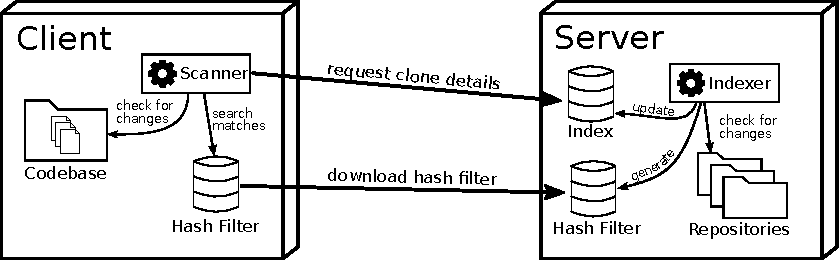
\includegraphics{figures/architecture_overview.pdf}
	\caption{Tool Architecture Overview}\label{fig:tool_architecture}
\end{figure}
\autoref{fig:tool_architecture} shows an overview of the tool's architecture.
The server has a pool containing repositories of open source software available on the Internet.
The index is a key-value store where the key is the hash of a chunk.
The Indexer on the server regularly updates the repositories and re-indexes changes as described in \ref{section:implementation/creating_index}.
In that process, it also calculates the hash filter which can be downloaded by clients.

The client has a codebase which is watched by a scanner.
The scanner normalizes, groups statements and hashes those groups the same way the server does.
It then uses the resulting hash to search for copy-pasted code.
For that, the client sends the hash to the server, which looks up the value stored in the index using the hash as the key.
If a match could be found for the hash, the server responds with the origin of the corresponding chunk.
The client can use a hash filter as described in \autoref{section:implementation/creating_index/hash_filter} to reduce the amount of requests to the server and speed up the scanning process.
The hash filter can also be used as an offline solution by the client for finding sections of code in its codebase, where there is a high probability of copied code.

\section{Creating the Index}\label{section:implementation/creating_index}
This section describes the process which is done to create the index.
First, the code which should be indexed is normalized file-by-file.
For each file, the code is parsed and split into tokens.
A token represents a small part of the code such as a symbol, keyword, identifier, literal or comment.
The tokens then are normalized as described below.
Now the tokens are aggregated into statements.
The tool then passes over the resulting list of statements using a sliding window to group together a chunk of code, which consists of several consecutive statements.
The amount of statements in a chunk influences the precision of a match, since longer chunks also require longer matches.

The resulting chunks could be used to find similar code segments.
Hashing the chunks with a hash function reduces the space needed to store the information.
As a hash function, MD5 is used, since it offers both, speed and high collision resistance.
\autoref{fig:normalization} shows the complete processing of an input file.

A relational database may reduce the size of the store, because redundancy can be removed.
However, tests showed that even with bulk inserts, the creation of the database is more than 50 times slower than using a key-value store.
In this work RocksDB was used as a key-value store implementation, since it has proven to be very fast and space efficient.

\begin{figure}[h]
	\centering
	\begin{minipage}{1.2\linewidth}
		\begin{minipage}{0.35\linewidth}
			\scriptsize
			\lstinputlisting[language=C++]{data/buffer.c}
		\end{minipage}
		\begin{minipage}{0.23\linewidth}
			\scriptsize
			\begin{lstlisting}
			AVBufferRef * create uint8_t * data , ... !\tikzmark{bgnFir}!
			AVBufferRef * ref = NULL !\tikzmark{bgnSec}!
			AVBuffer * buf = NULL !\tikzmark{bgnThi}!
			buf = av_mallocz sizeof * buf
			if ! buf
			return NULL !\tikzmark{trmFir}!
			buf -> data = data !\tikzmark{trmSec}!
			buf -> size = size !\tikzmark{trmThi}!
			buf -> opaque = opaque
			atomic_init & buf -> refcount , 1
			...
			\end{lstlisting}
			
			%			\begin{tikzpicture}[overlay, remember picture]
			%			\drawBrace[.6em]{bgnFir}{trmFi}{Example xshifted.};
			%			\drawBrace{bgnSec}{trmSec}{Example annotation.};
			%			\drawBrace{bgnThi}{trmThi}{Another example.};
			%			\end{tikzpicture}
			
		\end{minipage}
	\end{minipage}
	\caption{Normalization Process}\label{fig:normalization}
\end{figure}

\subsection{Normalization}\label{section:implementation/creating_index/normalization}
The normalization step removes irrelevant information and by that, concentrates on the essential features of the code.
The parsing of code into tokens already does the first part of normalization by removing formatting.
After that, irrelevant tokens like access modifiers, import or include statements, comments or symbols like brackets or semicolons are removed.
The tokens which are left contain the main portion of information relevant for comparison of two sequences of code.
Since the tool should uncover mainly directly copied code, no further normalization is done.
In early tests, additionally normalizing identifiers like variable names showed many false positives for variable initializations e.g. in the beginning of methods.

\subsection{History Analysis}\label{section:implementation/creating_index/history_analysis}
As mentioned in section \ref{section:requirements/detecting_old_version}, it is important to also index old versions of the reference system.
The server regularly pulls changes form the open source repositories on the Internet.

To keep the index up to date and still keep information about older versions of the file, changed files are re-indexed.
For that, the server normalizes the new version of the file the same way as described before, groups it into chunks and hashes those chunks.
The resulting hashes are then inserted into the key value store.
If a hash already exists and links to a file with the same location, the old link is replaced with the new one.
This ensures, that a hash always points to the latest version of a file.
When files are deleted, nothing is changed in the key value store.

Instead of rescanning the whole file, only the chunks which have changed could be scanned.
However, the locations of hashes for chunks which did not change also have to be updated  in order to keep the latest version of a file in the index.

Changes to the repository can be seen in different granularity.
A fine granularity would be commit based.
On the one hand, this would ensure that the index contains the files' content at any given point in time.
On the other hand, the amount of changed files is huge with that and indexing large projects may take quite long.
First tests with a commit-based approach on the Linux kernel's master branch showed that a complete indexing would take several days to finish.
Note here that the Linux kernel code is a special case, since its master branch has more than 600000 commits on it.
Nonetheless, this test showed that commit based may be to slow for productive use.
Therefore, a tag based approach is used:
For each tag found in the reference system's repository, a re-index is triggered.
All changed files since the last tag are re-indexed again and the key-value store is updated as described before.

\subsection{Hash Filter}\label{section:implementation/creating_index/hash_filter}
It is expected, that most of the calculated hashes of a target system can not be found in the index.
Instead of having to send a request for every hash to the server, a better option would be a local copy of the index for faster lookup.
However, since the index may contain key-value pairs for billions lines of code, it is huge.
Distribution of the index to clients is a challenge, especially since the index has to be updated regularly.

With a table of all hashes contained in the index, the client would be able to lookup whether a hash is in the index and only has to send a request to the server in this rare case.
This could significantly speed up the analysis, since only hashes which actually are in the index would be looked up.
On the server-side this also reduces the load.

The size of the hash table is the amount of hashes times 128 bits which is the length of a MD5 hash.
Hashing with MD5 reduces the entropy of a chunk to about 128 bit of a ideal hash function.
Since lossless compression is expected not to reduce the size of the hashtable by much, lossy compression could be used.
One great way of reducing size of hash table with low false-positive probability is a BloomFilter.

To store a value, a BloomFilter uses multiple hash functions to hash a value\cite{bloom1970filter}.
It uses the resulting hash values as indexes to set bits of a bit array to 1.
To find out whether a value is stored in the BloomFilter, the value is hashed with the same hash functions as for storing a value.
Again, hash values are used as indexes.
If all values inside the bit array defined by the indexes are set to 1, the value is stored in the BloomFilter with a high probability.
If one or more of the bits are not set, the value is guaranteed not in the filter.
For the tool developed in this work, the values inserted into the BloomFilter are the hashes of the chunks.

%TODO: "By making a sparse Bloom filter using 48 bits per element but only 3 hash functions, one can compress the result down to less than 16 bits per item with high probability) and decrease the false positive probability by roughly a factor of 2. @Mitzenmacher, Michael; Upfal, Eli (2005), Probability and computing: Randomized algorithms and probabilistic analysis S.10

The advantage here is the small size of the filter.
However, the compression is lossy, because there is a certain probability for false positives.
The probability is depending on the size of the bit array, the number of inserted values and the number of used hash functions, but when kept at an optimum, grows almost (due to discrete number of hashing functions) linearly with the number of insertions.
Since it is not possible to remove values from the filter, it has to be recalculated every time the index changes.

It is also possible to only use the filter to find potential copied code.
This however, does not allow the client to find the origin for a potential match.
	
\section{Searching Copied Code}\label{section:implementation/searching_copied_code}
The client has a codebase which should be searched for copied code.
To do so, it normalizes the code in question, groups statements and hashes them as described in \autoref{section:implementation/creating_index}.
%TODO Activity diagram: client <-> server
% TODO calculate probability of final false positive

\section{Future Work / Extensibility}\label{section:implementation/extensibility}
%TODO Extension points for future development? Web-Interface for code-add-request, Suggestions for linking libraries (gradle, ...)
\begin{itemize}
	\item Use Cuckoo-Filter \cite{fan2014cuckoo} instead of Bloom-Filter. Better performance in low false-positive probability with many items
	\item Optimize normalization: Method based?, block-based => switch methods/structs/enums positions
	\item Assess matches: Load file(s) from server, do more comparison (With a difftool token based on methods/blocks, to prevent reordering of methods not detected)
\end{itemize}
% !TeX root = ../main.tex

\chapter{Implementation}\label{chapter:implementation}
This chapter describes details about the prototype implementation of the tool, which is written in Java.

\section{Index Creation}\label{section:implementation/index_creation}
One goal of this work is the ability to find slightly modified code.
The idea followed here is to choose the number of statements in a chunk low to react on modified, added and removed statements.
The number of statements also has to be high enough to find license infringements as defined in \autoref{section:preliminaries/infringement}.
After several tests, 5 statements per chunk seemed reasonable.

For tokenization, existing code from the work of \cite{heinemann2014teamscale} is used.
Normalization is done by iterating over all tokens and removing rather irrelevant tokens like access modifiers, brackets, the java final or the C atomic keywords.
The stream of tokens is split into statements by language dependent tokens marking the end of a statement like semicolons or curly braces in Java or C/C++.
Include or import statements are removed.
In early tests, additionally normalizing identifiers like variable names showed many false positives for variable initializations e.g. in the beginning of methods or classes.
An example for the normalization of some sample code can be found in figure \ref{fig:normalization}\todo{Finalize figure, Java code instead?}.

\begin{figure}[h]
	\centering
	\begin{minipage}{1.2\linewidth}
		\begin{minipage}{0.35\linewidth}
			\scriptsize
			\lstinputlisting[language=C++]{data/buffer.c}
		\end{minipage}
		\begin{minipage}{0.23\linewidth}
			\scriptsize
			\begin{lstlisting}
			AVBufferRef * create uint8_t * data , ... !\tikzmark{bgnFir}!
			AVBufferRef * ref = NULL !\tikzmark{bgnSec}!
			AVBuffer * buf = NULL !\tikzmark{bgnThi}!
			buf = av_mallocz sizeof * buf
			if ! buf
			return NULL !\tikzmark{trmFir}!
			buf -> data = data !\tikzmark{trmSec}!
			buf -> size = size !\tikzmark{trmThi}!
			buf -> opaque = opaque
			atomic_init & buf -> refcount , 1
			...
			\end{lstlisting}
			
			%			\begin{tikzpicture}[overlay, remember picture]
			%			\drawBrace[.6em]{bgnFir}{trmFi}{Example xshifted.};
			%			\drawBrace{bgnSec}{trmSec}{Example annotation.};
			%			\drawBrace{bgnThi}{trmThi}{Another example.};
			%			\end{tikzpicture}
			
		\end{minipage}
	\end{minipage}
	\caption{Normalization Process}\label{fig:normalization}
\end{figure}

\todo{Problem with single statements in if/while/for without braces}
One emerging problem here are \texttt{if}, \texttt{while}, \texttt{for} or other blocks, which can be written with or without curly braces in the case of a single statement in the body.
Since the end of a statement is recognized by curly braces or semicolons as described above, a block with curly braces and a single statement is seen as multiple statements, one without the braces is seen as a single statement.
This may prevent copied code from being detected by the tool, when the braces are added or removed in the target system.
Since normalizing this case is rather complicated, it is ignored in this work.

A relational database can reduce the size of the store, because redundancy can be removed.
However, tests showed that even with bulk inserts, the creation of the database is more than 50 times slower than using a key-value store.
In this work RocksDB was used as a key-value store implementation.
As a hash function, MD5 is used, since it offers both, speed and high collision resistance.

As described in section \ref{section:approach/creating_index}, the key for an entry in the key-value store is the MD5 hash of a normalized chunk of code.
Since chunks with the same hash may be found in several locations, the value is a list of locations, where the chunk can be found.
For the prototypical implementation, the list for a value is serialized in JSON
Figure \ref{fig:json_serialization} shows a simplified example.

\begin{figure}[h]
	\centering
	\begin{lstlisting}
		{
			[
				{
					"project": "referenceProjectName",
					"path": "src/component/ClassA.java",
					"start": 8262,
					"end": 8993,
					"revision": "ac89b33fe7a..."
				},
				{
					"project": "otherProjectName",
					"path": "src/component/SomeOtherClass.java",
					"start": 2689,
					"end": 3053,
					"revision": "893afe7b3ca..."
				},
				...
			]
		}
	\end{lstlisting}
	\caption{Simplified JSON String representing a sample value for an entry in the key-value store}\label{fig:json_serialization}
\end{figure}

\section{History Analysis}\label{section:implementation/history_analysis}
Copied code of a system may origin from a previous version of a reference system.
Modern version control systems like git, subversion or mercurial enable user to go back in time and extract any version of a source code file from the system's repository.
In this work, this is used to add old versions of source code files to the index in order to find code which has been copied from an older version of the reference system.

Versions of a repository can be seen in different granularity.
A very fine granularity would be considering every commit as a different version of the system.
On the one hand, indexing every commit would ensure that the index contains a files' content at any given point in time.
On the other hand, the number of versions and therefore the amount of files to index is huge.
Indexing large projects like that may take quite long.

First tests with a commit-based approach on the Linux kernel's master branch showed that a complete indexing would take several days to finish.
Note here that the Linux kernel code is a special case, since its git repository contains more than 600000 commits at the time of writing.
Nonetheless, this shows that commit based may be to slow for productive use.
Furthermore, changes between two commit often are minor and may not be relevant, e.g changing a constant or literal.

Instead, the implementation of this work is using a tag based approach.
First, all tags found in the reference system's repository are extracted and sorted.
After that, starting at the first tag, all files present at that point in time are indexed as described in section \ref{section:implementation/index_creation}.
Following up, for each tag in order, the changed files relative to the previous tag are indexed again.
All changed files since the last tag are re-indexed again and the key-value store is updated as described in section \ref{section:approach/creating_index/history_analysis}.

\subsection{Quick Scan}\label{section:implementation/history_analysis/quick_scan}
When a new reference project should be added to the index, no versions of the project have been scanned yet.
One way of indexing the versions defined by the available tags is to start with the tag with the oldest commit, get all files of that version and index them as described before.
After that, the next version defined by the next tag in order by date of the commit the tags are pointing to, could be indexed.

Instead of this approach indexing old to new versions of the reference project, a quicker indexing technique can be used.
The problem here is that a file often is only changed in some lines, but the bigger part of the file stays untouched.
When indexing is done from old to new, each chunk, which has not been changed, can already be found in the database pointing to the previous indexed version of the file and has to be updated.
The old entry has to be deleted and the new entry pointing to the new version of the file has to be added.
Instead, when indexing new to old versions, the entry for the chunk does not have to be changed and simply can be dropped.
This ensures that each hash in the database is pointing to the latest version of a file.

\subsection{Updating the Database}\label{section:implementation/history_analysis/update}
As explained before, the index should be updated regularly in order to find the latest copied code.
Therefore, the latest indexed version of each reference project has to be tracked.
To update the index on the server, all repositories are updated to include the latest changes.
After that, for each reference project, tags are extracted and sorted as mentioned before.
Now, instead of traversing the tags chronologically reversed, i.e from new to old tags based on the date of the commit they are pointing to, tags are scanned chronologically, i.e. from old to new.
This time, all hashes already in the database and pointing to the same file path are updated instead of dropped.

\subsection{Sorting Tags}\label{section:implementation/history_analysis/sorting_tags}
For this work, a prototype implementation for git was done.
Using git tags to get periodic snapshots of a reference system showed some difficulties during testing.

Especially for bigger projects, tags are not always sorted chronologically.
Using the tagging date may not be always accurate, since tags can be added in hindsight.
Instead, the commit date of the commit a tag is pointing to is used to sort the tags chronologically.
However, this can cause huge amounts of changed files between two tags in some cases.
One example is illustrated in \autoref{fig:tag_sort}.
For different versions, different branches exist, e.g. \texttt{v1} and \texttt{v2}.
Tags are added for every release of a version, e.g. \texttt{v1.6}.
The indexing progresses from tag to tag in chronological order by the commit date of the commit the tag is pointing to.
As the example shows, the progress is jumping between the branches causing many changed files and therefore heavily slowing down the indexing.
To compete with that, different branches of the projects where scanned as different projects.
One example is the Openjdk project, where jdk8 and jdk9 are developed on two different branches.
For each of the major versions, a copy of the project was indexed, only regarding tags, which belong to the specified version.
This could easily be done using a regular expression matching.

Another emerging problem is tags not pointing to a commit.
In git, a tag can point to any git object, such as e.g. a commit, a tree or another tag.
To deal with this circumstance, all tags not pointing to a commit where ignored during indexing.

\begin{figure}[h]
	\centering
	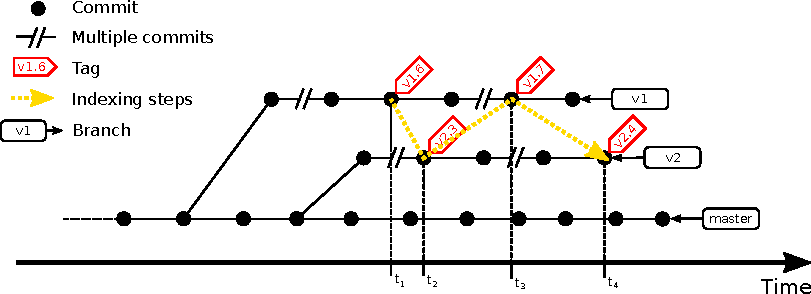
\includegraphics{figures/tag_sort.pdf}
	\caption{Tags on different branches causing many changes}\label{fig:tag_sort}
\end{figure}

Still, several problems persist: 
Clock skew amongst commiters may result in inaccurate sorting of tags and therefore could result in chunks remaining in the index not pointing to the latest version of a file.
Keeping only references to chunks of the latest version of a file seems also to be a problem when searching for copied code on a client, since matches may be scattered over multiple versions of a file, because some chunks may point to a newer version of the file instead of the version the section of code actually was copied from.
Those problems could be solved by keeping all chunks in the index, which have the same hash and are pointing to different versions of a file.
However, this would increase the size of the database drastically.
The size of the filter would not increase, since not the amount of hashes, but the amount of values a single hash is pointing to is increased.
In the prototypical implementation of the approach presented in this work, this is ignored, since scattered matches are aggregated as described in \ref{section:implementation/finding_matches}.

A better solution to sorting tags would be a branch based approach:
Every branch is followed and snapshots of the reference system are either made periodically or with the use of tags.
This may not only increase accuracy, but also indexing speed, since less files change between two versions (see \autoref{fig:tag_sort}).

\section{Hash Filter}\label{section:implementation/hash_filter}
With hash filter, this work refers to an algorithm, which can decide whether a element is part of a set with the help of a data structure which represents parts of the index.
A simple approach would be to extract the set of all hashes from the index and shorten each one of them to reduce size, e.g. instead of 128bit per hash, only the first $i$ bits are used.
Hashes which are equal in the first $i$ bits but different in the remaining bits have the same shortened hash.
One hash may actually be part of the set of hashes and therefor part of the index, whereas the other may not.
With this approach a decision can not be made with absolute precision.

The probability $p$ of a false positive, which is the probability for the list of shortened hashes containing an entry for the first $i$ bits of a hash, but the hash not being part of the index can be calculated as follows:\\
First the possibility for a hit $p_h$ is determined:
\begin{equation}
	p_h=\frac{n}{2^i}
\end{equation}
with the number of hashes $n$ and the length of a shortened hash $i$, given that hashes are uniformly distributed.
The probability $p_c$ for the hash being part of the index can be calculated as follows:
\begin{equation}
	p_c=\frac{n}{2^{128}}
\end{equation}
The resulting probability $p$ for a false positive can be calculated as follows:
\begin{equation}
	\begin{split}
		p&=p_h\cdot (1-p_c) \\[10pt]
		&= \frac{n}{2^i}\cdot \left(1-\frac{n}{2^{128}}\right)
	\end{split}
\end{equation}

The main disadvantage of this approach is that with increasing number of hashes $n$ in the list, the amount of bits per hash has to rise in order to keep the probability low.
For a probability of 0,01\% for a billion hashes the required length $i$ of a shortened hash would be 44 bit:
\begin{equation}
	\begin{split}
		p&=\frac{n}{2^i}\cdot \left(1- \frac{n}{2^{128}}\right) \\[10pt]
		2^i&=\frac{10^9}{10^{-4}}\cdot \left(1- \frac{10^9}{2^{128}}\right) \\[10pt]
		i&=\log_2\left(10^{13}\cdot \left(1- \frac{10^9}{2^{128}}\right)\right) \\[10pt]
		i&\approx 43,19 \rightarrow 44 \text{ bit per hash}
	\end{split}
\end{equation}
This would result in 
\begin{equation}
	44\text{ bit} \cdot 10^9 = 44\cdot10^9 \text{ bits} = 5,5 \text{ GB}
\end{equation}
\\
As mentioned before, in this work a Bloom Filter is used to decide, whether a hash is contained in the index.
A Bloom Filter is a probabilistic data structure which can decide, whether an element is part of a set with a small probability for a false positive.
It uses a bit array of size $m$ to store information about the values in the set.
The probability for a false positive can be calculated as follows \cite{fan2000summary}:
\begin{equation}\label{equ:false_positive_bloom}
	p=\left(1-\left(1-\frac{1}{m}\right)^{kn}\right)^k \approx \left(1-e^{-\frac{kn}{m}}\right)^k
\end{equation}
where $n$ is the number of hashes in the set, $m$ the number of bits in the Bloom Filter's bit array and $k$ the number of hash functions used, to store a value in the bit array.
The optimum number of hash functions to use, is defined as the $k$ which minimizes the probability of the false positive $p$.
To calculate the optimal $k$, which has to be positive, the approximation from equation \ref{equ:false_positive_bloom} can be used.\todo{How?}
\begin{equation}
	\begin{split}
		k&=\frac{m}{n}\ln(2)
	\end{split}
\end{equation}
When using a billion hashes for $n$ and a probability of 0,01\% as before, the size $m$ of the bit array needed for the optimum $k$ calculates as follows:
\begin{equation}
	\begin{split}
		m&=-\frac{n\ln p}{(\ln2)^2} \text{ bit} \\[10pt]
		&=-\frac{10^9\ln10^{-4}}{(\ln2^2)} \text{ bit} \\[10pt]
		&\approx 1,9\cdot10^{10} \text{ bit}=2,4\text{ GB}
	\end{split}
\end{equation}

Using a Bloom Filter instead of a list of shortened hashes to decide whether a hash is part of the index reduces the size of the filter, which has to be downloaded to less than a half for a billion hashes.
%TODO plot?
%\begin{figure}[h]
%	\centering
%	\begin{tikzpicture}
%		\begin{axis}[
%				samples=1000,
%				xmin=0,
%				xmax=1000,
%				ymin=0,
%%				ymax=1000000000,
%				xlabel={Number of Hashes in Millions},
%				ylabel={Filter Size in MB},
%			\addplot[domain=0:1200]{-(x*10^6*ln(0.0001)/((ln(2))^2))/8000000};
%		\end{axis}
%	\end{tikzpicture}
%	\begin{tikzpicture}
%		\begin{axis}[
%			samples=1000,
%			xmin=0,
%			xmax=1000,
%			ymin=0,
%			xlabel={Number of Hashes in Millions},
%			ylabel={Number of Hash Functions},
%		]
%		\addplot[domain=0:1200]{ln(2)*(-(x*ln(0.0001)/((ln(2))^2)))/x};
%		\end{axis}
%%	\end{tikzpicture}
%	\caption{Optimal Bloom Filter size in relation to stored hashes}
%\end{figure}

For the prototypical implementation, the Google Guava library's Bloom Filter implementation is used.
It features easy setup and an efficient way to store into and load the filter from a file.

\section{Scalability}\label{section:implementation/scalability}
The indexing process can be parallelized, which highly improves the indexing speed.
In this prototypical implementation, a thread pool with 16 threads is used.
For each version of a reference project, which should be scanned, a new indexing task is created for each file of that version.
The resulting tasks are then processed by threads of the thread pool.
This is done for each version of a project and for each project, resulting on 16 threads processing one version.

Here, it is important to not change the value of a hash by different threads at the same time since this may cause a race condition.
To compete with this, a Java HashSet was used to lock the hash currently being changed by a thread.

Another difficulty is the requirement to keep the latest version of a file in the index.
To keep it simple, projects only were index one version at a time.

Tests showed, that indexing was about 8 times faster using this approach compared to a single threaded run.
The process could be parallelized even more, by concurrently indexing multiple projects at the same time.
Also it may be possible to scan multiple versions of one project at the same time, when the index keeps  references to all versions of a chunk instead only an entry pointing to the latest version of that chunk (compare section \ref{section:implementation/history_analysis/update}).
However, during test, the machine already was at its limits using this approach, leaving those options open for distributed environments.

\section{Finding Matches}\label{section:implementation/finding_matches}
For this prototypical implementation, the networking between client and server is ignored.
Instead hashes are filtered using the bloom filter and looked up by directly accessing the database containing the index.

Referring to the definitions provided in section \ref{section:preliminaries/infringement/how_much_code}, a clone is considered an infringement, if a minimum of about 8 lines of code or, in the context of this work, statements are copied.
A chunk consists of 5 statements, therefore at least two chunks have to be copied, when a single statement has been modified like illustrated in figure \ref{fig:required_chunks_modified}.
This would total in 10 copied statements, since there are no overlapping chunks.
When no statement has been modified, a sequence of statements has to consist of at least 4 chunks to contain a total of 8 statements as illustrated in figure \ref{fig:required_chunks}.
Here, 4 consecutive chunks are copied resulting in 8 copied statements without gaps.

\begin{figure}[h]
	\centering
	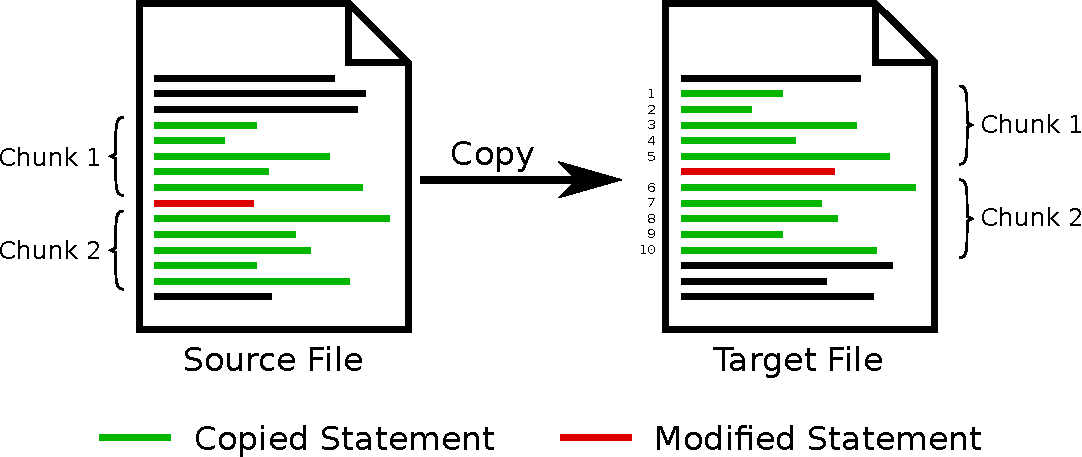
\includegraphics[width=0.9\linewidth]{figures/required_chunks_modified.pdf}
	\caption{Minimum required chunks for copied code with modification}\label{fig:required_chunks_modified}
\end{figure}

\begin{figure}[h]
	\centering
	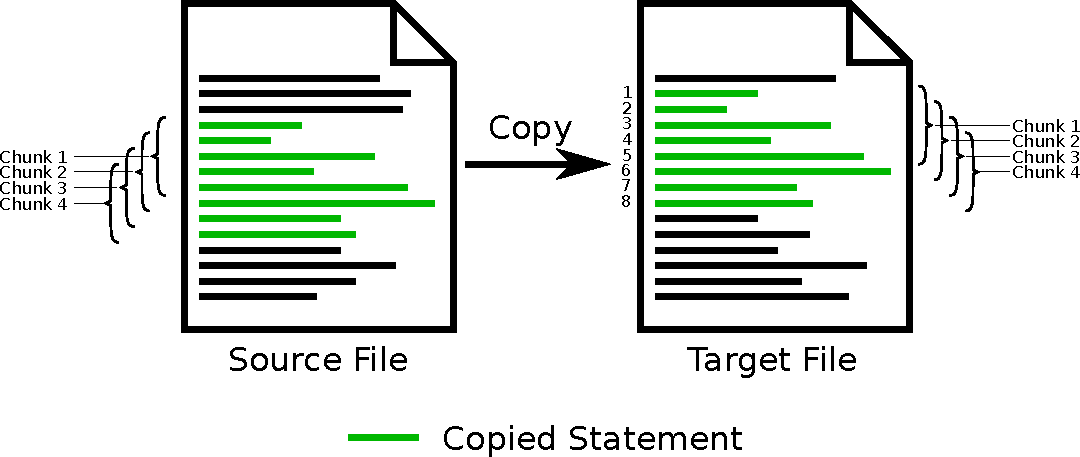
\includegraphics[width=0.9\linewidth]{figures/required_chunks.pdf}
	\caption{Minimum required chunks for copied code without modification}\label{fig:required_chunks}
\end{figure}

To compete with these limitations, for each file, chunks are extracted as described above.
The Hash Filter is used to decide whether a chunk is part of the index and therefore a match exists within the file.
If a file has less than 2 matching chunks, it can be ignored, since the minimum amount is two as explained above.
Otherwise, details about the matches are requested from the server by sending the list of hashes for chunks, which the filter marked as part of the index.
The server responds with a list of locations for each hash, or an empty list, if the hash is a false positive of the Hash Filter.

The client groups locations by reference project and path of the file.
Note here that the revision of the file a chunk is pointing at, is ignored in this step.
This makes sense, since locations always point to the latest revision of a chunk as described in section \ref{section:approach/creating_index/history_analysis}.

The client then merges consecutive matches, by iterating over the locations of a group and finding overlaps.
The amount of locations in a merged match is stored.
When merging, a small gap is allowed between two locations of the same group, to include modifications of copied code as described in section \ref{section:approach/creating_index}.
In the case of such a gap, the count of locations for the match is incremented by 4, since a possible modification has been detected and the actual length of the copied segment is equal to about 10 statements as it can be seen in figure \ref{fig:required_chunks_modified}.

Now the client can filter all matches which have a location count of less than 4 and remaining matches fulfill the required minimum length for a violation as described above.
\\
Continuous detection with e.g. every commit on a target system's codebase is possible.
The same steps as described above can be done for each changed file instead of the whole codebase.
% !TeX root = ../main.tex

\chapter{Evaluation}\label{chapter:evaluation}
To verify the capability of the approach proposed in this work, the prototypical implementation was tested.
The idea is to find out, whether the approach is capable of detecting copied code in a codebase and, by that, unveil license infringements.
For that purpose, 2000 GPL licensed projects were indexed using the prototypical implementation of the tool.
After that, other open source projects, which are licensed not compatible with GPL and therefore should not contain any of the GPL licensed code indexed before, where analyzed and emerging matches categorized.

This chapter describes the test setup evaluates timings, database sizes and findings.

\section{Test Setup}\label{section:evaluation/test_setup}
As a source for the projects to index, GitHub was chosen.
GitHub's REST API was used to generate a list of 1.000 GPL licensed Java and 1.000 GPL licensed C or C++ projects.
All of the projects were checked out locally resulting in sizes as shown in \autoref{table:locs}.

Indexing those 2.000 projects including their history took 15h on a consumer laptop with 16 GB of RAM and an Intel i7 2.6 GHz CPU with 4 cores and hyper-threading.
The indexing was done independently for Java and C/C++ generating two databases.
The resulting database sizes are 4 GB for Java and 33 GB for C/C++, the bloom filter's sizes are 55 MB and 147 MB for Java and C/C++.

Inspection of several indexed projects showed, the huge difference for the sizes can be justified in the amount of actual code in the repositories.
It seems like Java projects contain more images, binary files or other resources, compared to the C/C++ projects.
Also, the resulting count of chunks and corresponding amount of hashes indicates a lot of duplicated chunks and leads to the assumption that the increase of hashes is asymptotic relative to the growth of chunks.

\begin{table}[ht]
	\centering
	\begin{tabular}{l|rrrrr}
		& \textbf{Scanned Files} & \textbf{Lines of Code} & \textbf{Total size} & \textbf{Hashes} & \textbf{Chunks} \\ 
		\hline 
		Java & 836.555 & 57.834.764 & 94 GB & 23.773.065 & 35.069.633 \\
		C/C++ & 1.023.092 & 380.338.327 & 102 GB & 61.349.163 & 221.315.454 \\ 
	\end{tabular}
	\caption{Sizes of the 2.000 indexed projects}\label{table:locs}
\end{table}

After two weeks, the index was updated for both Java and C/C++ as described in \ref{section:implementation/history_analysis/update}.
Approximately one third of the reference projects contained one or more new tags which were indexed.
The update took a total of one hour including calculation of the bloom filter.
This shows that incremental updates of the index are worth the effort of implementation compared to re-indexing the reference projects from scratch.

After indexing those projects, several other projects, licensed not compatible with GPL, where analyzed for matches using the approach described in section \ref{section:implementation/finding_matches}.
\autoref{table:target_projects} shows the chosen target projects, their license and the lines of code of files written in the corresponding language.
To reduce the amount of irrelevant matches, generated code and third party code in libraries were excluded from the target projects during analysis.

\begin{table}[ht]
	\centering
	\begin{tabular}{l|llr}
		& \textbf{Name} & \textbf{License} & \textbf{Lines of Code} \\
		\hline 
		\parbox[t]{2mm}{\multirow{10}{*}{\rotatebox[origin=c]{90}{JAVA}}} 
		& IntelliJ IDEA & Apache 2.0 & 3.500.000 \\
		& Eclipse JDT Core & Eclipse Public License & 1.459.000 \\
		& Elasticsearch & Apache 2.0 & 711.000 \\
		& Eclipse JDT UI & Eclipse Public License & 685.000 \\
		& Facebook Buck & Apache 2.0 & 597.000 \\
		& Teamscale & Closed Source & 480.000 \\
		& Spring Boot & Apache 2.0 & 223.000 \\
		& Openfire & Apache 2.0 & 200.000 \\
		& Killbill & Apache 2.0 & 150.000 \\
		& JabRef & MIT & 125.000 \\
		\hline 
		\parbox[t]{2mm}{\multirow{10}{*}{\rotatebox[origin=c]{90}{C/C++}}} 
		& Chromium & BSD License 2.0 & 4.651.000 \\
		& ArangoDB & Apache 2.0 & 4.855.000 \\
		& Tensorflow & Apache 2.0 & 662.000 \\
		& Apple Swift & Apache 2.0 & 520.000 \\
		& Mesos & Apache 2.0 & 309.000 \\
		& Apache httpd & Apache 2.0 & 214.000 \\
		& RethinkDB & Apache 2.0 & 201.000 \\
		& Tesseract & Apache 2.0 & 147.000 \\
		& Bitcoin & MIT & 119.000 \\
		& Electron & MIT & 67.000 \\
	\end{tabular}
	\caption{Target projects used for testing, their license and LOCs in the corresponding language}\label{table:target_projects}
\end{table}

\section{Hash Filter Performance}\label{section:evaluation/hash_filter_performance}
The bloom filter can return false positives, thus, matches are expected even if no code has been copied from a reference project into the target project for large enough projects.
Those matches - called false positive filter matches (FPFM) in the remainder of this work - are expected to occur once for roughly every 10.000 statements in the target project, since the probability for a false positive of the bloom filter is calculated to be 0,01\%. 

Table \ref{table:unfiltered_findings} lists results regarding amount of analyzed chunks as well as false and true positive matches.
Columns are defined as follows:
\begin{description}
	\item[Target System] The name of the target system
	\item[Files] Number of files of the target project, which match the corresponding language (Java or C/C++) and are therefore analyzed.
	\item[Chunks] Resulting amount of chunks extracted from the target system.
	\item[FPFM] False Positive Filter Matches as described above.
	\item[True Positives] Amount of actual matches, which could be found in the index and their relative amount in comparison to all chunks extracted from the target system.
	\item[Requests] Amount of requested match details. Note here that files with less than two matches are ignored as described in section \ref{section:implementation/finding_matches}.
\end{description}

\begin{table}[ht]
	\centering
	\begin{tabular}{l|lrrrrr}
		 & \textbf{Target System} & \textbf{Files} & \textbf{Chunks} & \textbf{FPFM} & \textbf{True Positives} & \textbf{Requests} \\ 
		\hline 
		\parbox[t]{2mm}{\multirow{10}{*}{\rotatebox[origin=c]{90}{JAVA}}} 
		& IntelliJ IDEA & 35.398 & 1.570.170 & 183 & 8.134 (0,5\%) & 8.035 \\
		& Eclipse JDT Core & 1.829 & 267.130 & 29 & 510 (0,2\%) & 509 \\
		& Elasticsearch & 5.560 & 414.448 & 45 & 1.105 (0,3\%) & 1.004 \\
		& Eclipse JDT UI & 2.736 & 274.040 & 29 & 482 (0,2\%) & 444 \\
		& Buck & 5.150 & 261.605 & 21 & 575 (0,2\%) & 548 \\
		& Teamscale & 5.463 & 185.648 & 21 (0,011\%) & 458 (0,247\%) & 434 \\
		& Spring Boot & 3.756 & 94.935 & 11 & 1.010 (1,1\%) & 967 \\
		& Openfire & 1.572 & 121.775 & 15 & 2.106 (1,7\%) & 2.084 \\
		& Killbill & 1.477 & 79.118 & 13 & 550 (0,7\%) & 539 \\
		& JabRef & 1.389 & 72.052 & 5 & 204 (0,3\%) & 183 \\
		\hline 
		\parbox[t]{2mm}{\multirow{10}{*}{\rotatebox[origin=c]{90}{C/C++}}} 
		& Chromium & 14.241 & 364.126 & 53 & 16.951 (4,7\%) & 16.912 \\
		& ArangoDB & 1.096 & 135.291 & 8 & 571 (0,4\%) & 569 \\
		& Tensorflow & 1.207 & 50.382 & 3 & 59 (0,2\%) & 56 \\
		& Apple Swift & 848 & 56.386 & 11 & 14 (0,0\%) & 13 \\
		& Mesos & 341 & 64.090 & 6 & 18 (0,0\%) & 15 \\
		& Apache httpd & 529 & 126.936 & 18 & 949 (0,7\%) & 949 \\
		& RethinkDB & 91 & 8.664 & 0 & 2.906 (33,5\%) & 2.905 \\
		& Tesseract & 559 & 82.946 & 10 & 27 (0,0\%) & 29 \\
		& Bitcoin & 491 & 57.847 & 5 & 97 (0,2\%) & 97 \\
		& Electron & 342 & 6.846 & 1 & 0 (0,0\%) & 0 \\
	\end{tabular}
	\caption{Amount of files and chunks as well as true and false positives caused by the Hash Filter and the resulting requested chunk details}\label{table:unfiltered_findings}
\end{table}

This result shows that the Hash Filter is reducing the required lookups to a fraction.
Load on the server can be greatly reduced and analysis of a target system's code therefore is a lot quicker.

The analysis took less than 20 seconds even for the biggest projects not including networking.
In a real world scenario, this will be slower, since communication with the server will add additional delays.

Requesting the locations for each hash passing the Hash Filter individually, causes a lot of requests with high overhead caused by creating single network packets.
Additional authentication on the server may be required to control access further slowing down the analysis.
Instead, sending hashes in batches may be a better solution.

\newpage
\section{Detection of License Infringements}\label{section:evaluation/detecting_infringements}
As the previous section shows, matches have to be filtered, in order to remove false positives and matches, which are not relevant in the context of license infringement.
Aggregation and filtering is done as described in \autoref{section:implementation/finding_matches}.

Based on the license definitions in section \ref{section:preliminaries/infringement/relevant_licenses}, each match is manually inspected and grouped into one of the following categories:
\begin{description}
	\item [Accidential Clones (AC)]
		Matches which are similar by \glqq accident\grqq, e.g. generated code, interface implementations, declarations of structs/enums, switch-case blocks, table data especially present in C/C++.
	\item[Otherwise Licensed Code (OLC)]
		Code which is actually copied from the reference project or originates from a common source licensed under a permissive license or is public domain.
		If the copied code is under permissive license, attribution is done correcty and therefore, this is not a license infringement.
		Note here that code can also be copied into the reverse direction in the context of this evaluation, since analyzed target projects are licensed in a way, where they can be copied to GPL licensed code with attribution.
	\item[Copied, but not Attributed (CNA)]
		This marks the use of permissive licenses and therefore is the same as otherwise licensed code, but not attributed correctly by the target project.
		The severity of the violation is depending on the license of the source, the length of the copied segment and its similarity.
		Those violations can be fixed by correctly attributing the source of the code.
	\item[License Infringement (LI)]
		Code which has been copied from a reference system licensed under a restrictive license and is violation due to the target's license.
\end{description}

AC can be seen as a false positive of the approach, whereas OLC detects code, which has been copied, but the license of the code is not violated.
Even though OLC does not violate a license, detection of such code still may be of interest, since using a library instead of copying the code into the codebase can be the better alternative \cite{heinemann2012effective}.
In general, those two cases are not marking violations.

CNA on the other hand, marks a violation of the license, because the code has not been attributed correctly, but the significance of such a violation may not be very high.
Copied code categorized as LI may even be attributed correctly, but still is a violation of the copied code's license.

\subsection{Counting Matches}
A scanned target system file can have multiple matches for a chunk, since clones also exist between and within reference systems.
Therefore, in the following evaluation, matches are counted on the target file and only the most relevant concatenated matches of the reference files are regarded.
\autoref{table:scan_results} shows the results of manually categorizing each match.
A match is a relation between a file of the target system to the best match of a file in a reference system, indicating a high similarity.

If a target file has multiple sections of copied code, which \textit{does not overlap} and is from multiple other files (e.g. common in utils code), each match in the target file is counted once.
Figure \ref{fig:match_counting} shows an example, where multiple sections of code are copied from \texttt{Reference File 1} to the \texttt{Target File}.
This is counted as one match.
There is also one coherent block of code copied from \texttt{Reference File 2} to the \texttt{Target File}, which is also counted as a match.
The resulting total count of matches for the \texttt{Target File} in this example is two.

\begin{figure}[h]
	\centering
	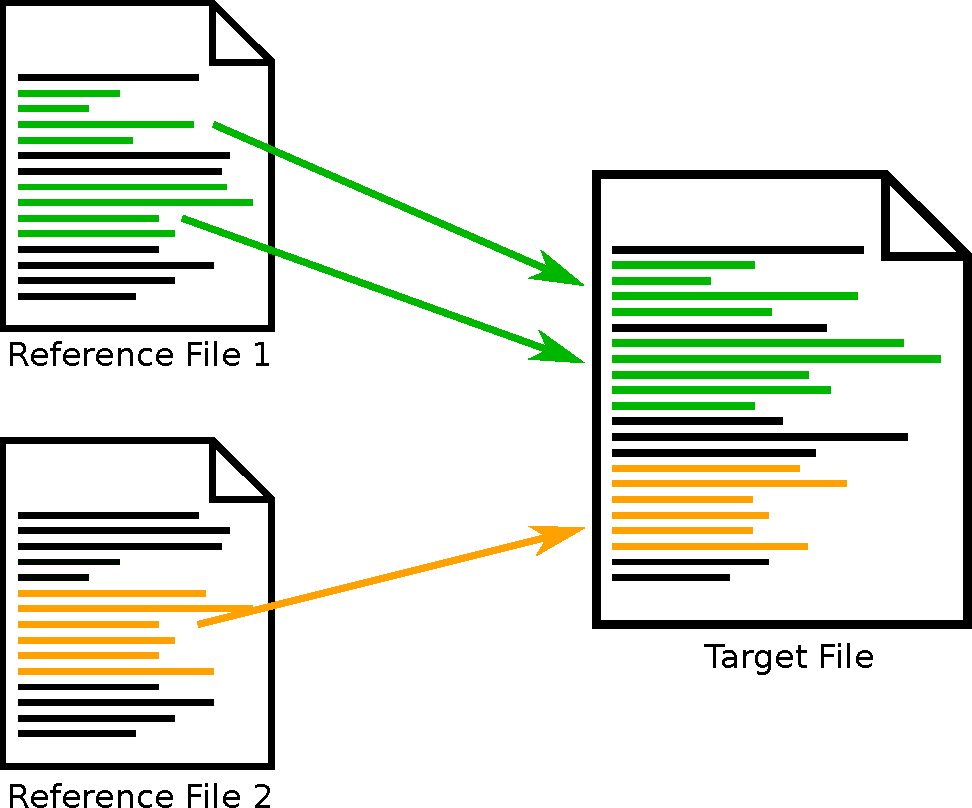
\includegraphics[width=0.7\linewidth]{figures/match_counting.pdf}
	\caption{Illustration of match counting}\label{fig:match_counting}
\end{figure}

\newpage
\subsection{Results and Findings}
The results in table \ref{table:scan_results} are twofold.
On the one hand, it shows that finding license infringements is possible.
On the other hand, the amount of overall detected matches prevails the amount of relevant matches by far.
This is due to many accidental clones (AC), which are caused by e.g. interface implementations or tables, as well as otherwise licensed code (OLC) due to the fact that most licenses of target projects allow copying of code into a codebase licensed under GPL.
Therefore, many of the hits for OLC are caused by code of the target project being found in the reference project.

\begin{table}[ht]
	\centering
	\newcolumntype{R}[1]{>{\raggedleft\arraybackslash}p{#1}}
	\begin{tabular}{l | l rrrr}
		& \textbf{Name} & \textbf{AC} & \textbf{OLC} & \textbf{CNA} & \textbf{LI} \\
		\hline 
		\parbox[t]{2mm}{\multirow{10}{*}{\rotatebox[origin=c]{90}{JAVA}}} 
		& IntelliJ IDEA & 86 & 21 & 11 & 7 \\
		& Eclipse JDT Core & 17 & 8 & 0 & 0 \\
		& Elasticsearch & 13 & 3 & 4 & 3 \\
		& Eclipse JDT UI & 3 & 19 & 0 & 0 \\
		& Facebook Buck & 11 & 7 & 0 & 0  \\
		& Teamscale & 12 & 3 & 1 & 2 \\
		& Spring Boot & 19 & 6 & 0 & 0 \\
		& Openfire & 20 & 9 & 5 & 0 \\
		& Killbill & 20 & 2 & 0 & 0 \\
		& JabRef & 3 & 2 & 0 & 1 \\
		\hline 
		\parbox[t]{2mm}{\multirow{10}{*}{\rotatebox[origin=c]{90}{C/C++}}} 
		& Chromium & 16 & 429 & 0 & 0 \\
		& ArangoDB & 1 & 5 & 0 & 0 \\
		& Tensorflow & 2 & 0 & 0 & 0 \\
		& Apple Swift & 2 & 0 & 0 & 0 \\
		& Mesos & 1 & 0 & 0 & 0 \\
		& Apache httpd & 5 & 13 & 0 & 0 \\
		& RethinkDB & 0 & 29 & 0 & 0 \\
		& Tesseract & 2 & 1 & 0 & 0 \\
		& Bitcoin & 0 & 6 & 0 & 0 \\
		& Electron & 0 & 0 & 0 & 0 \\
	\end{tabular}
	\caption{Target projects and categorized matches}\label{table:scan_results}
\end{table}

\subsubsection*{General Findings}
For Java, the approach found several infringements, for C/C++ no LI nor CNA were found.
This may be explained, by many of the C/C++ target projects being of organizations, which have their own library codebase.
Manual investigation in the findings leave the impression that C/C++ developers are more careful in copying code correctly and attributing copied code correctly.

Sometimes, the decision whether a match is actually copied code (OLC or CNA depending on the license) or just accidential clones (AC) is visible in the comments.
When both sides have a high similarity in the comments, the probability for the code being copied increases significantly.
Still, removing comments when normalizing code for comparison is advisable, since comments often are removed or added.

The match supplied by the tool sometimes was not the actual origin of the code.
However in many times, the suggested matches could give hints on the origin of the code and combined with further searching the Internet, the originating source could be determined.
This process is very hard to automate and manual inspection is required nonetheless, since the severity of the infringement has to be assessed.
For some rare cases, even searching for implementations of the specific problem on the Internet did not help to find the originating source.
For such cases, the code was seen as CNA, since no attribution was made and the code may be a potential infringement.
This also shows that indexing one reference project often includes several other projects (with different licenses), since sometimes, dependencies are copied into the codebase of a reference project.

Infringements not only could be found in the target system.
Sometimes, the original file header was replaced by the GPL header of the reference system, which for many licenses is a violation.
Those cases are not regarded in this test, but still show that the problem targeted in this work exists.

Some of the selected reference projects are forks of one of the target projects.
Examples are Eclipse JDT Core and the Overture tool\footnote{\href{https://github.com/overturetool/overture}{https://github.com/overturetool/overture} (09.01.2018)} or Chromium and the OBS Studio project\footnote{\href{https://github.com/jp9000/obs-studio}{https://github.com/jp9000/obs-studio} (09.01.2018)}.
Almost all matches of RethinkDB were caused by copied code from RapidJSON\footnote{\href{https://github.com/Tencent/rapidjson}{https://github.com/Tencent/rapidjson} (09.01.2018)}.

\subsubsection*{Accidential Clones (AC)}
Mostly, AC findings are caused by interface implementations, structs and enumerations used for communication with APIs or table definitions.
One example of a common AC is shown in figure \ref{fig:ac}.
Here, the Java specific \texttt{hashCode} and \texttt{equals} methods cause a match.
Method generators supplied by the used IDE may have caused the high similarity.
\begin{figure}[htpb]
	\centering
	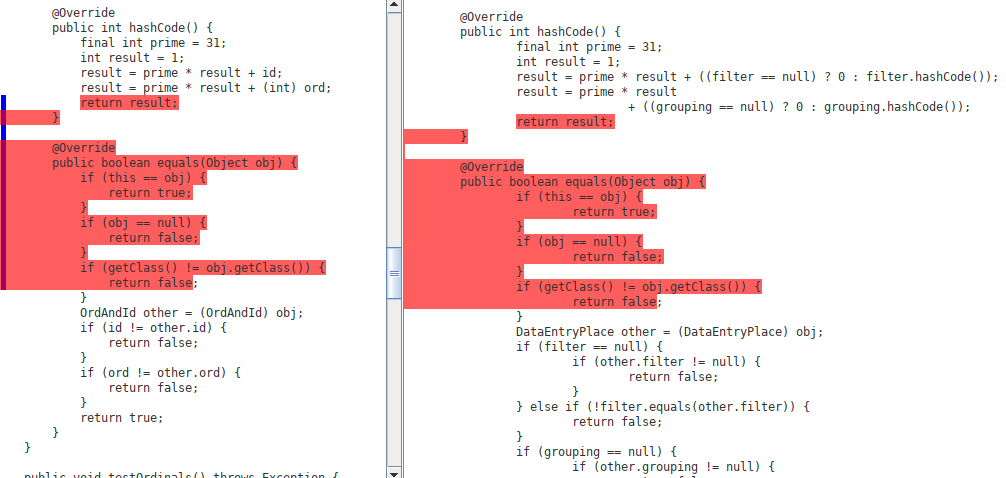
\includegraphics[width=\linewidth]{figures/ac.png}
	\caption{Example for AC. Left target, right reference code}\label{fig:ac}
\end{figure}

\newpage
\subsubsection*{Copied but not Attributed Code (OLC)}
OLC had many matches both for Java and C/C++.
Either code was attributed correctly like the example in figure \ref{fig:olc_attributed} or the code can be copied without attribution like in the case of code under public domain like the example in \ref{fig:olc_public_domain} shows.
Findings like those are not license infringements.
However, they may be of interest, since third party code can be monitored and code could be linked instead of copied.

Some of the selected reference projects are forks of one of the target projects.
Examples are Eclipse JDT Core and the Overture tool\footnote{\href{https://github.com/overturetool/overture}{https://github.com/overturetool/overture} (09.01.2018)} or Chromium and the OBS Studio project\footnote{\href{https://github.com/jp9000/obs-studio}{https://github.com/jp9000/obs-studio} (09.01.2018)}.
Almost all matches of RethinkDB were caused by copied code from RapidJSON\footnote{\href{https://github.com/Tencent/rapidjson}{https://github.com/Tencent/rapidjson} (09.01.2018)}.

A reference system being licensed under a specific license does not cause all code files of that system are actually licensed as such.
Resolving the actual license of a file can be very hard, since headers often do not contain any information on the file's license.
\begin{figure}[h!]
	\centering
	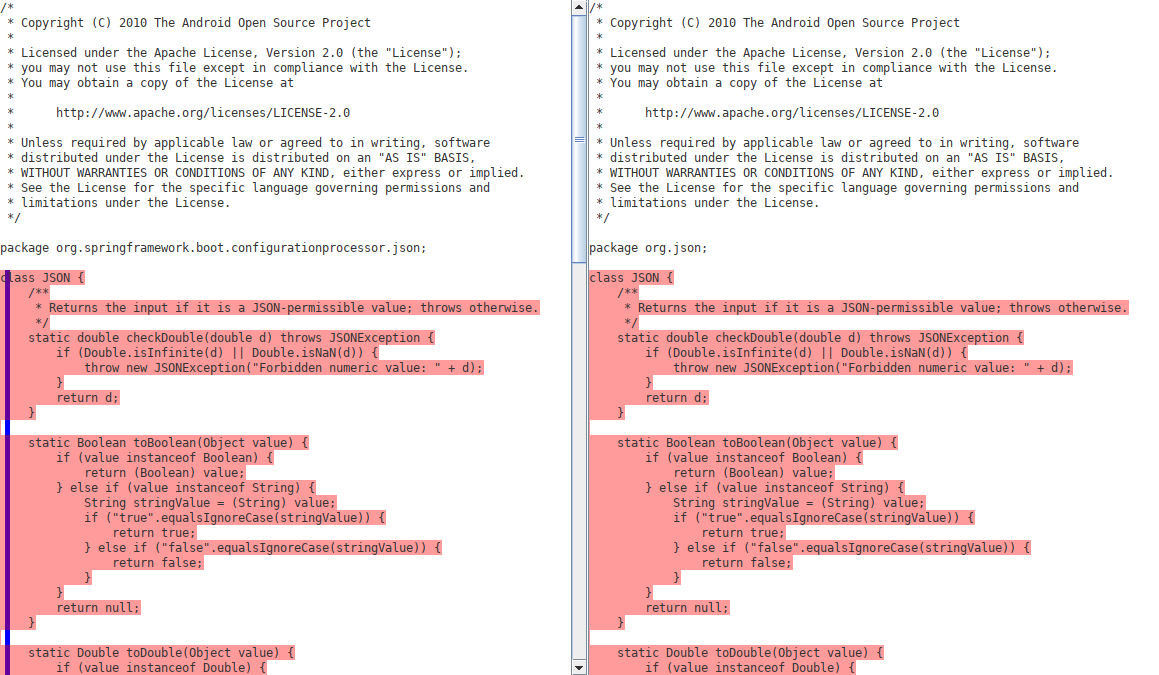
\includegraphics[width=\linewidth]{figures/olc_attributed.png}
	\caption{Example for correctly attributed OLC. Left target, right reference code}\label{fig:olc_attributed}
\end{figure}
\begin{figure}[h!]
	\centering
	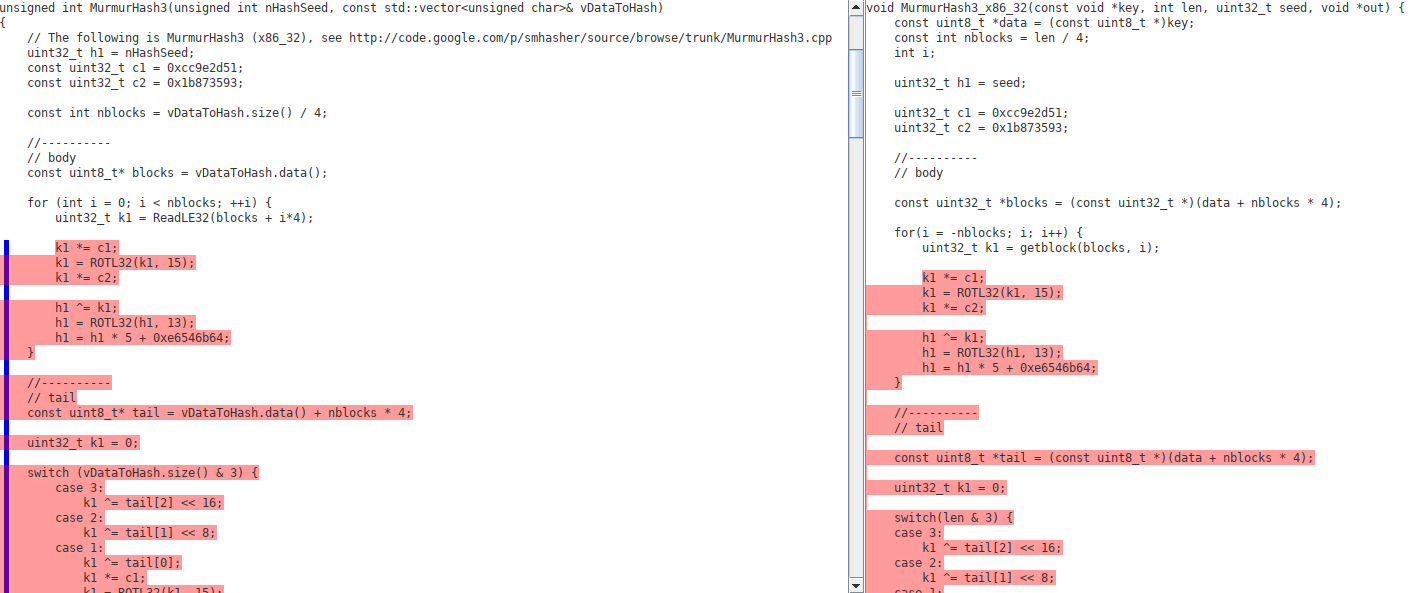
\includegraphics[width=\linewidth]{figures/olc_public_domain.png}
	\caption{Example for public domain code being categorized as OLC. Left target, right reference code}\label{fig:olc_public_domain}
\end{figure}

\newpage
\subsubsection*{Copied but not Attributed Code (CNA)}
In many cases, attributing the origin of copied code is not done correctly, as manual inspection showed.
Figure \ref{fig:cna} shows an example for CNA, where hundreds of lines were copied, but no attribution was made.
The original file header containing the license information including the terms and conditions was replaced by the target project's file header.
This causes a violation of the licenses terms, since attribution has to be made according to the reference file's license.
\begin{figure}[htpb]
	\centering
	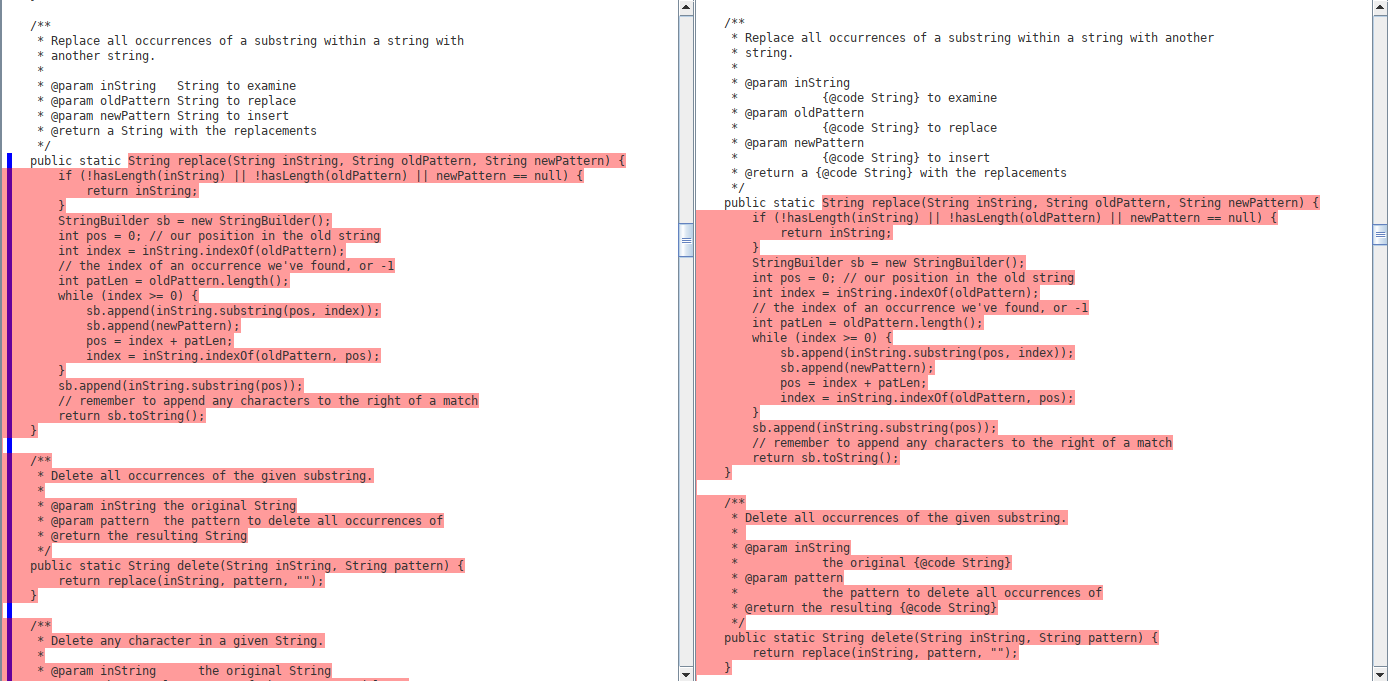
\includegraphics[width=\linewidth, trim={1mm 3,8cm 0 0}, clip]{figures/cna.png}
	\caption{Example for CNA. Left target, right reference code}\label{fig:cna}
\end{figure}

\newpage
\subsubsection*{License Infringment (LI)}
Cases categorized as LI are violations of the GPL, where code is copied from a GPL licensed file to the target system.
Almost all cases found are caused by adoption of classes from the Java Development Kit (JDK).
The license of both, OpenJDK's and Oracle JDK's source code files is not compatible with permissive licenses like Apache or MIT, nor with closed source.
It seems like many developers are not aware of this.
On example of such an infringement can be found in figure \ref{fig:li}, where a method of a class in the JDK was modified.
The code is then licensed under Apache 2.0 which is not compatible with GPL.
Instead, the code should be licensed under GPL.
This example shows that even small amounts of copied code which cause violations can be detected using the tool, although modifications were made.

Many of those cases are rather small and may not be prosecuted when uncovered.
Nonetheless, those findings show that the problem targeted in this work exists and can be detected using the approach presented in this work.
\begin{figure}[htpb]
	\centering
	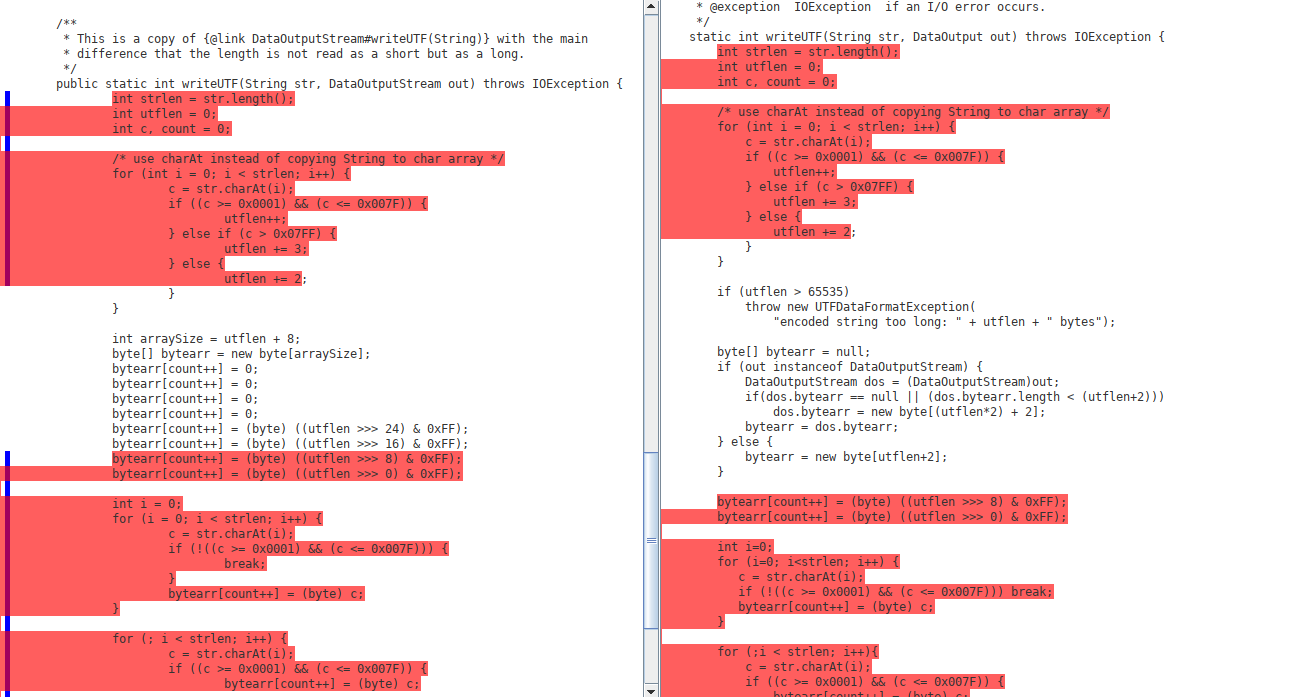
\includegraphics[width=\linewidth]{figures/li.png}
	\caption{Example for LI. Left target, right reference code}\label{fig:li}
\end{figure}

\subsection{Testing Recall}
Asserting the recall of clone detection tools is difficult.
Benchmarks like the work of Svajlenko et al. \cite{svajlenko2014towards} can give insight on the recall performance.
Analyzing this work with such a benchmark go beyond the scope of this work and may even be not suitable, since the benchmark is testing for similar code constructs, which can be refactored for reuse to reduce redundancy and enhance software quality.
In contrast, the tool presented in this work tries to find code which has a high similarity and can be argued for being copied.

\section{Confidentiality}
The tool may be used for closed source target systems.
One key issue for companies is confidentiality regarding own source code.
Uploading code to a server maintained externally to the company may not be conform with the company's data privacy policies.

The approach presented in this work is only sending hashes which represent information relevant for identifying chunks.
In theory, this should restrict flow of information about the source code to a minimum and conclusions about the code can not be made.
However, when the code for a hash is known on the server side, i.e. a match for a hash is found, the server knows the code for the hash on the client.
If enough matches are found, the server may be able to reconstruct parts of the source code.
Still, information about the source code leaking from the client to the server is very limited.
% !TeX root = ../main.tex

\chapter{Future Work}\label{chapter:future_work}
The approach is scalable and can be heavily distributed, which may even make it possible to index and track the history of most of the open source code available on the Internet.
However, there is a lot of room for improvement:

\paragraph{Distributed Server Architecture}
Since this work proposes a client-server architecture, it is important to provide a reliable service to a huge amount of clients.
Therefor, distributing the index on several machines is desirable for load balancing.
This could easily be done by distributing the database onto the machines whenever the index is updated.

It may also be advisable to group reference projects by license or other parameters like origin of the code (GitHub, Bitbucket, Debian source repositories, \dots).
Pairs of servers and filters responsible for a group of reference projects could be created.
This would result in multiple small hash filters and enables clients to only choose filters of their interest, further reducing the size of the filter a client has to download and keep up to date.
The requests resulting from matches in the filter on the client side then have to be routed to the server responsible for the corresponding group of reference projects.

Distributing the workload can also speed up the indexing process, when updates are triggered (see \autoref{section:implementation/scalability}).

\paragraph{Branch Based History Analysis}
The accuracy of the history analysis could be improved significantly.
As explained in \autoref{section:implementation/history_analysis/sorting_tags}, the problem is sorting the tags of a reference project's repository in the correct order without producing huge amounts of changed files between two revisions and slowing down the indexing process.
A better approach would be to start with important branches and find tags on the way back to the root of the commit tree.
Especially for big codebases with many branches, it may be important to filter branches, which are only used to implement features and are later on merged with a release branch.
Since this heavily depends on the policy of the individual reference projects, manual inspection would be required or an approach to automate the filtering has to be developed.

\paragraph{Reducing Amount of Accidental Clones (AC)}
With the current state of the approach, findings have to be inspected manually for violations, which sometimes can be a very time consuming process, since the actual origin of the code may not be part of the reference systems.
Also, many of the found matches are not relevant, since either they are accidental clones and are not actually copied or the code in question does not cause any licensing issues.
Results and insights emerging from the development of the tool presented in this work show that solving those problems is difficult.
This mostly is caused by the peculiarity and individuality of reference projects and their licensing models.

As mentioned in \autoref{section:evaluation/detecting_infringements} one of the reasons for accidental clones are getters and setters.
Removing those during the normalization process would probably reduce the amount of accidental clones.

Another source of accidental clones are declarations done for API compliance outside of methods.
Testings done in \autoref{chapter:evaluation} showed, that most copied code is located inside the body of methods on both sides, the reference and target system.
Concentrating the comparison of code on code blocks such as methods, structs, enumerations or other language specific constructs, could reduce the amount of such false positives.

Clients could also blacklist matches, which are irrelevant.
Matches which are blacklisted by many clients could then be sorted out on the server side and excluded from results and the filter.

\paragraph{Hash Filter Improvements}
The original idea for a Bloom filter is already more than 40 years old \cite{bloom1970filter}.
There has been a lot of research to improve the filters performance and reduce its size.
Tulsiani et al. found out that \glqq making a sparse Bloom filter using 48 bits per element but only 3 hash functions, one can compress the result down to less than 16 bits per item with high probability and decrease the false positive probability by roughly a factor of 2\grqq \ \cite{tulsiani2013probability}.
Compared to the example calculation done in \autoref{section:implementation/hash_filter}, a filter containing one billion hashes would be about 2 GB, reducing the size by 17\%.
The work of Fan et al. proposes a filter structure called Cuckoo-Filter, which has a better performance when the filter contains many items. and needs a low false positive probability.
This would fit the requirements for a filter in this work.
% !TeX root = ../main.tex

\chapter{Conclusion}\label{chapter:conclusion}
The tests conducted in \autoref{chapter:evaluation} showed that licensing issues can be found and may help software developers to prevent license violations.
Using a Bloom filter to reduce the amount of required requests can speed up the analysis and reduce the load on the server to a fraction.
In 25\% of the analyzed projects, issues with licensing could be found which shows that the problem targeted in this work exists.

Due to the difficulty of finding the correct origin of copied code, discovering the actual license is very hard, if possible at all.
This restrains the approach from automatically determining the license and deciding whether a violation is present.
Also, there are many licenses from which open source developers can choose.
Owners of open source software can even create a new license if existing ones are not suiting their project.
It is even possible to establish a special agreement between the copyright owners of source code which adds even more confusion to the license-jungle.

Beside that, the tool may not only be used to find licensing issues, but also enable developers to monitor used libraries and third party code.
This information can be used to link libraries instead of copying the code.
In the long run, this could improve software quality, since maintaining of third party code could be simplified and vulnerabilities caused by outdated code can be fixed.


\appendix{}

\microtypesetup{protrusion=false}
\listoffigures{}
\listoftables{}
\microtypesetup{protrusion=true}
\printbibliography{}

\end{document}
